\documentclass{article}

% Language setting
% Replace `english' with e.g. `spanish' to change the document language
\usepackage[francais]{babel}

% Set page size and margins
% Replace `letterpaper' with`a4paper' for UK/EU standard size
\usepackage[a4paper,top=2cm,bottom=2cm,left=3cm,right=3cm,marginparwidth=1.75cm]{geometry}

% Useful packages
\usepackage{amsmath}
\usepackage{amsfonts}
\usepackage{fancyhdr}
\usepackage{graphicx}
\usepackage[T1]{fontenc}
\usepackage{float}
\usepackage{subfig}
\usepackage[colorlinks=false, allcolors=blue]{hyperref}

\title{
    \underline{MAT 41 02} \\
    Apprentissage Non Supervisé - Application sur la base de données MNIST
}
\author{Charles FARHAT}

\pagestyle{fancy}
\renewcommand{\headrulewidth}{0.2pt}
\renewcommand{\footrulewidth}{0.2pt}
\fancyhead[L]{}
\fancyhead[R]{\textit{Apprentissage Non Supervisé - MNIST}}
\fancyfoot[C]{\thepage}
\fancyfoot[R]{TP MNIST - Charles Farhat}



\begin{document}
\maketitle

\begin{figure}[h]
    \centering
    
\includegraphics[scale=0.22]{Images/1024-1318.png}
\end{figure}


\newpage
\vspace*{\stretch{1}}
\begin{center}

    \tableofcontents
    %Pour qu'une section ne soit pas prise en compte dans la table des matières il suffit d'écrire 
    %\section*{Titre de la section}
\end{center}
\vspace*{\stretch{1}}


\newpage


\section{Introduction}
Ce rapport fait suite à la réalisation du cours \textit{Introduction aux méthodes de classifications non supervisées} du modules \textbf{MAT 4102} de Télécom SudParis. \newline
Dans ce rapport il sera question de la très connue base de données MNIST, ce TP porte donc sur la plus classique introduction à de l'apprentissage machine : la classification de chiffres écrits à la main.  

La spécificité tiens à l'approche qui sera utilisée pour la classification : nous chercherons à la réaliser à partir de méthodes usuellement appliquées à des problèmes non supervisés. 
Par ailleurs, il est imposé d'utiliser les algorithmes \textit{Kmeans} et \textit{Kmedoids}, le contenu portera donc sur la comparaison des résultats de ces deux algorithmes dans différents contextes.

\vspace{2mm}
Il est également demandé à ce que ce rapport soit succint. Nous considérons donc que certains des principes et fonctionnements de bases des deux algorithmes sont connus et nous nous concentrerons uniquement sur ce qui a été apporté.


\newpage

\section{Découverte des algorithmes et première approche}
\vspace{4mm}

Le but de ce TP n'est pas de développer à proprement parler les algorithmes Kmeans et Kmedoids mais de les analyser. Toute références à ces deux fontions sera issue de la librairie \textit{Scikit Learn},  \url{https://scikit-learn.org/stable/}. La base de données utilisée est quant à elle issue de la librairie \textit{Pytorch}. Elle est composée de $70000$ matrices représentants des chiffres de 0 à 9 sur des images en niveaux de gris de 784 pixels (28*28, 1 dimension, pixels valants 0 à 255). 

\begin{center}
  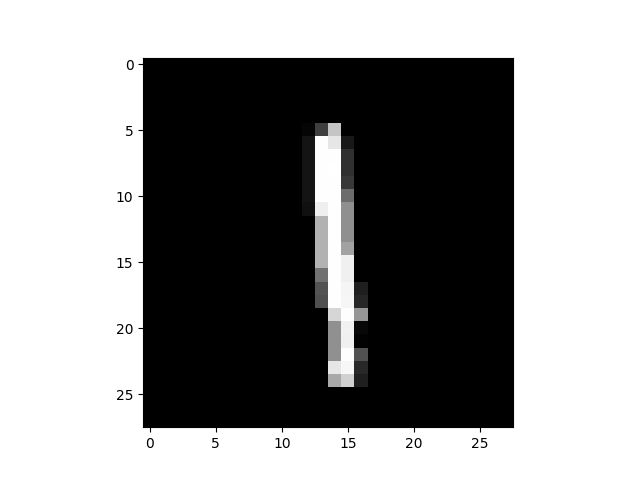
\includegraphics[width=0.3\textwidth]{"./Images/1.png"}
  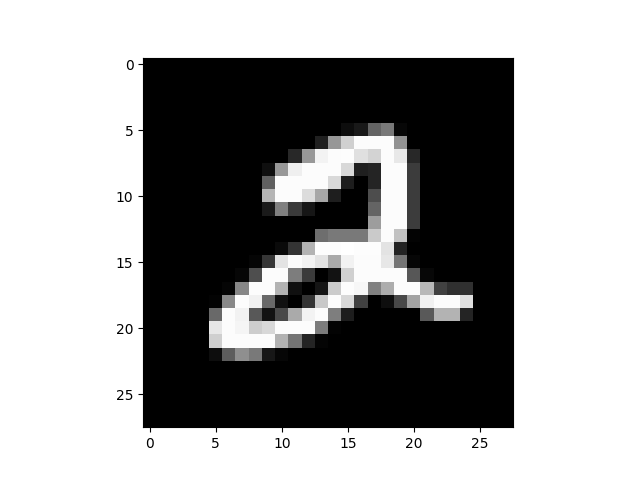
\includegraphics[width=0.3\textwidth]{"./Images/2.png"}
  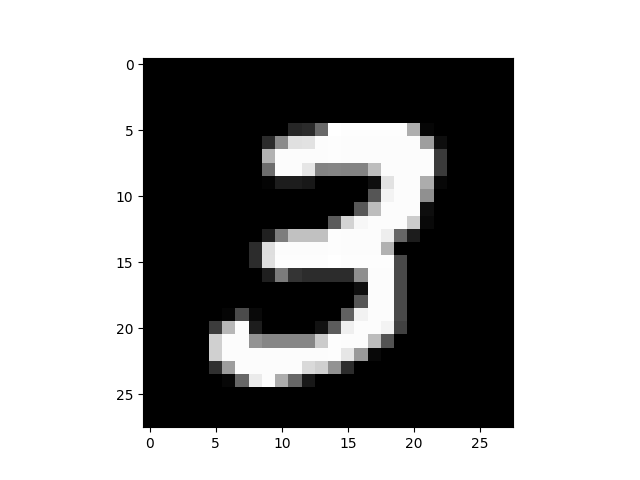
\includegraphics[width=0.3\textwidth]{"./Images/3.png"}
\end{center}

%Quelques images issues de la base de données.


\textit{Dans toute notre étude nous utiliserons les paramètres par défault proposés par sklearn,  notamment $n\_init$ et $max\_iter$ qui correspondent respectivement au nombre d'initialisationx à considérer (Kmeans étant fortement non convexe, son état initial a un grande influence sur le résultat final) et au nombre d'itérations maximales (pour le calcul de position des barycentres) s'il ne semble pas y avoir convergence "rapide" de l'inertie. \newline Les raisons sont d'abord que le rapport demande une présentation succinte mais également parce que la détermination des hyperparamètres est surtout un enjeux pour l'augmentation des performances, ce qui n'est pas l'objectif ici.} 

\subsection{Observation et Premiers résultats}

\subsubsection{Observation}

La première chose qu'il tient à faire, surtout dans le cas d'apprentissage non supervisé, est de chercher à représenter les données, de rendre visuel ce que nous cherchons à trier. classifier. Nous sommes ici chanceux : même si l'on supposait ne pas connaître la classe de chaque matrice à l'avance, visualiser des images de cette simplicité (niveau de gris) et en déduire des tendances est une tâche relativement aisée. \\
Quelques remarques peuvent rapidement être formulées après une première observation du dataset : 

\begin{enumerate}
    \item Les images ne sont pas centrées.
    \item L'immense majorité des images contient une bordure de noir lorsque l'on s'approche des bords. Cette bordure varie de 3 à 7/8 pixels.
    \item Certaines images contiennent principalement des niveaux de gris aux endroits représentants leur chiffre.
\end{enumerate}

Que déduire de ces observations ? Pour y répondre il convient de s'intéresser d'abord au fonctionnement des algorithmes.

Aux yeux de Kmeans et Kmedoids nos images sont simplements des vecteurs de 784 coordonnées. Le but des deux programmes est de déterminer des frontières permettants de séparer ces vecteurs en $n \in \mathbb{N}^*$ groupes, le tout en minimisant un critère appelé \textit{Inertie}. 
\\

Il est donc sensé de penser que plus les données qui sont présentées en entrée  à l'algorithme seront "facilement" séparables, meilleure la classification sera. \newline
\textit{Par 'facilement' il est entendu que les données similaires sont proches et les autres sont éloignées, par rapport à une norme.} \\

Or comme nous venons de le mentionner, presque toutes les images admettent des pixels noirs lorsque nous nous rapprochons des positions extrêmes. Une telle propriété n'est pas discrimante et donc d'aucune utilité pour les deux algorithmes, c'est pourquoi nous proposons donc de réduire les image à des matrices 22*22 en supprimant les 3 premières et dernières lignes, ainsi que les 3 premières et dernières colonnes. \\

Une fois ce premier traitement réalisé, nous avons certes réduit la quantité d'informations disponibles (vecteurs de 784 coordonnées à vecteurs de 484 coordonnées) mais nous avons surtout augmenté la qualité de nos données. Ce type de transformation est souvent recherché en apprentissage machine car il permet de réduire le temps de calcul tout en augmentant les performances. 

Un autre type de transformation particulièrement prisé est celui de l'augmentation de données. \newline
Cette fois, plutôt que de chercher à discriminer en supprimant des données inutiles nous allons chercher à augmenter les informations portées par celles déjà présentes. Le fait que certaines images présentent majoritairement des niveaux de gris implique que pour une même représentation matricielle (les indices des pixels valants 0 et dex pixels non nuls ont la même position) la distance (disons euclidienne) entre l'image en noir et blanc et l'image en niveau de gris serait non négligeable et pourrait fausser la classification des algorithmes. \\

Pour palier ce problème il est possible d'utiliser un algorithme de lissage : si un pixel est en dessous d'une valeur seuil on le diminue à 0, à l'inverse s'il est supérieur on l'augmente à 255. Sans toucher à la dimension du problème nous rapprochons ainsi les vecteurs similaires et éloignons ceux différents.


\begin{figure}[H]
    \centering
    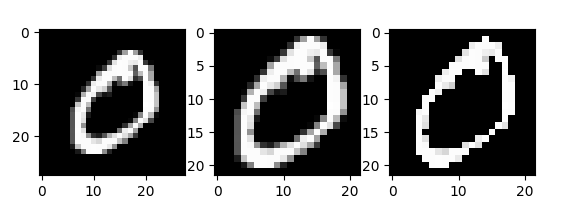
\includegraphics[width=\textwidth]{"./Images/pre_pro_0.png"}
    \caption{\label{fig:lign1}Évolution de l'image au fil des transformations}
\end{figure}

\subsubsection{Premiers résultats}

Une fois les programmes introduits dans la partie précédente fonctionnels nous pouvons passer à l'implémentation des fonctions coeurs de ce TP : Kmeans et Kmedoids. \\

\textit{Remarque : Dans le cas de MNIST les données sont déjà comparables à l'état brut, il ne semble donc pas particulièrement important de les standardiser. D'autant plus que le but est davantage d'introduire à de nouvelles notions que d'arriver à des performances intéressantes (d'autant plus qu'il s'agit de MNIST...). Nous diviserons tout de même tous les pixels par 255 pour les normaliser, afin d'avancer sur des grandeurs plus petites.}

\begin{figure}[H]
    \centering
    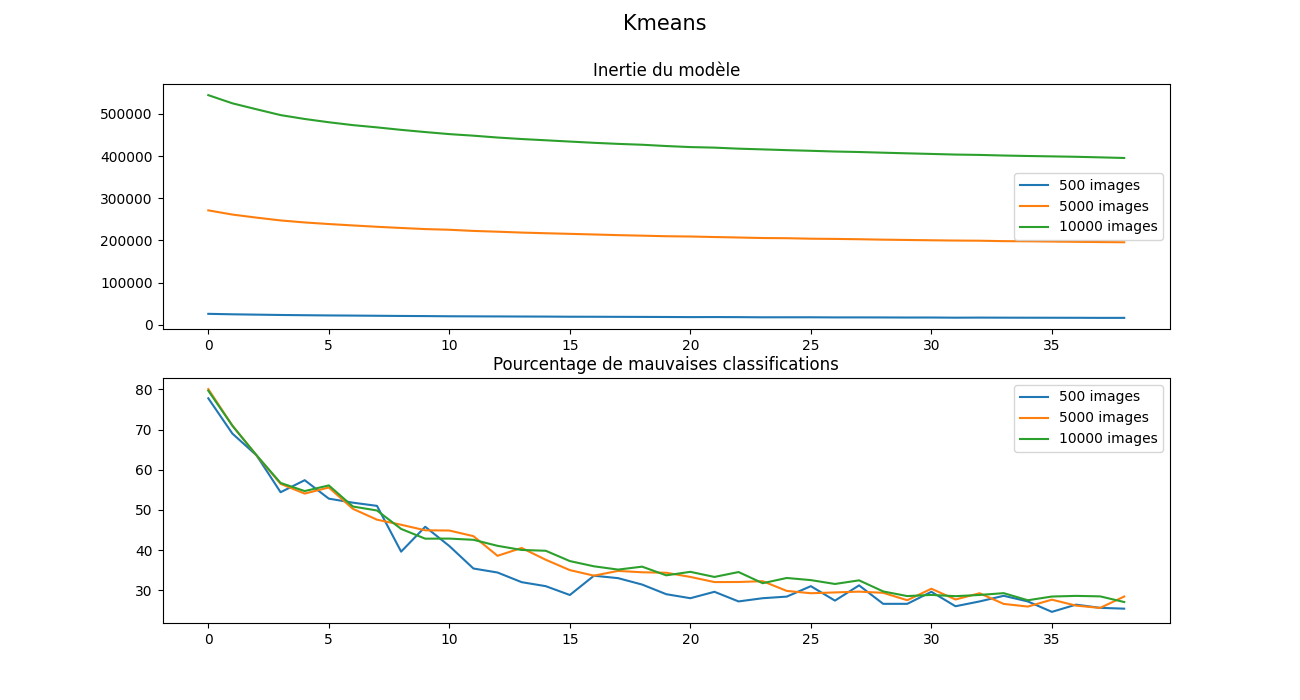
\includegraphics[width=0.8\textwidth]{"./Images/Kmeans_no_prepo_erreur.png"}
    \caption{Inertie et erreurs de classification pour Kmeans en fonction du nombre de Cluster (2 à 50)}
    \label{fig:kmeansnopreproerr}
    
\end{figure}

\begin{figure}[H]
    \centering
    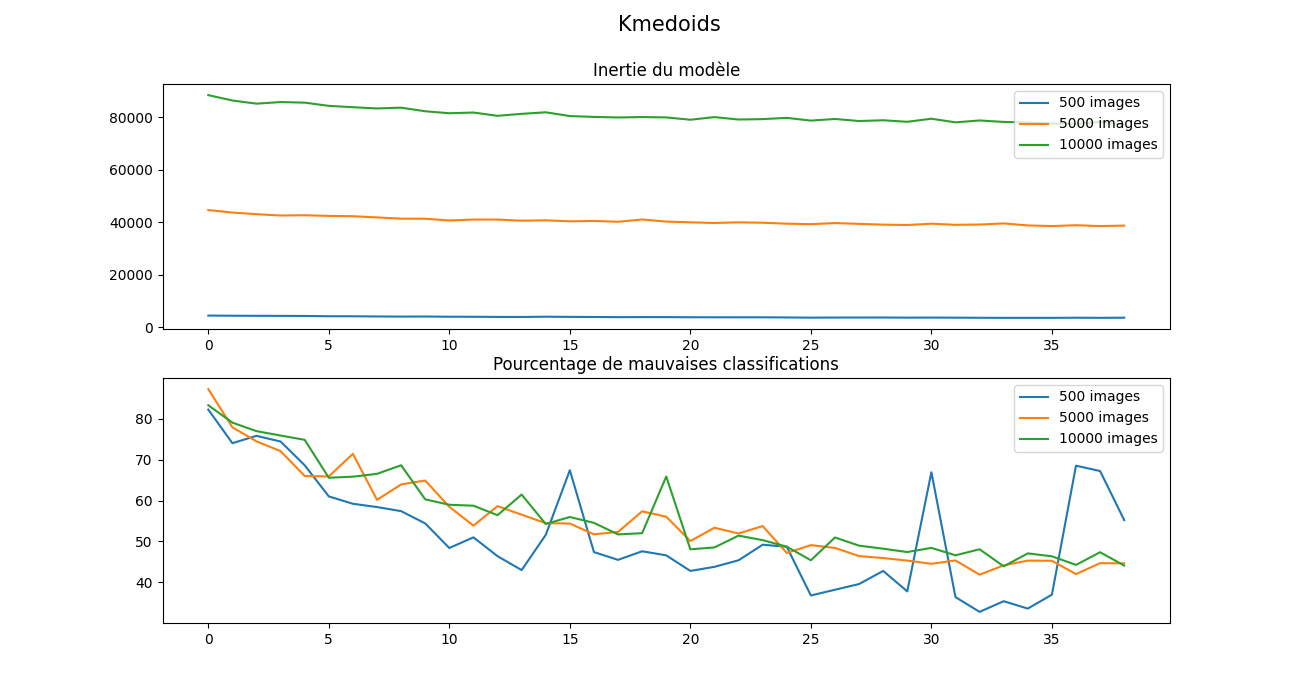
\includegraphics[width=\textwidth]{"./Images/Kmedoids_no_prepo_erreur.png"}
    \caption{Inertie et erreurs de classification pour Kmedoids en fonction du nombre de Cluster}
    \label{fig:kmedoidspapapa}
\end{figure}
\vspace{2mm}


\textit{Dans le cas où nous définissons plus de 10 clusters nous utilisons une fonction de pré-traitement qui associe une étiquette (entre 0 et 9) à chaque cluster. Pour décider nous choisissons d'associer l'étiquette de la classe la plus représentée (par rapport aux vraies étiquettes) dans chacun de ces clusters. Nous calculons ensuite l'erreur à partir de ces 10 représentations.} \\

Quelques remarques : 
\vspace{1mm}

\begin{itemize}
    \item L'inertie diminue avec le nombre de cluster, ce qui est cohérent.
    \vspace{1mm}
    
    \item Le pourcentage d'erreur diminue aussi (de manière moins stable avec Kmedoids) avec le nombre de clusters. Un même chiffre pouvant s'écrire de plusieurs façons, (sept avec et sans barre par exemple) l'association finale en 10 clusters présentée précédemment permet de les classer à la fin comme un même chiffre. Que cette erreur diminue avec le nombre de clusters est donc également cohérent.
    \vspace{1mm}
    
    \item Dans le cadre de 5000 images et une réduction/lissage pour chaque image l'algorithme Kmedoids converge bien plus rapidement que Kmeans. (En moyenne sa convergence 10 fois plus rapide). Cette tendance diminue en revanche avec la taille du dataset.
    
\end{itemize}
\vspace{2mm}

Les pourcentage d'erreurs de classifications augmentent cependant avec la taille de la base de données, il serait intéressant de chercher à savoir si cette tendance se confirme avec davantage de clusters (jusqu'à 250) et d'images. (Ce qui sortirait du cadre du présent rapport, qui est simplement une introduction à l'algorithme).

\vspace{1.5mm}
\textit{Dans la littérature on trouve que les applications sérieuses de Kmeans utilisent 200 clusters pour la classifications de MNIST, les résultats que nous obtenons tendent bien dans ce sens.}


\subsection{Nouvelles métriques}

L'information la plus regardée dans le cas d'une étude sérieuse serait très probablement le pourcentage moyen d'erreurs. Or il n'est possible de l'obtenir qu'à condition de travailler sur une base de données étiquettées.  \\

Dans la pratique les algorithmes d'apprentissage non supervisés sont très rarement utilisés sur des bases de données étiquettées, nous n'aurions donc pas accès à cette erreur moyenne. L'inertie  présentée dans la partie précédente est un indicateur certe intéressant pour ce type de situation mais son analyse seule (valeur et vitesse de convergence) manque d'information, c'est pourquoi il existe d'autres indicateurs permettants de décider si une classification est non seulement 'bonne' mais également 'correctement paramétrée'.  \\

Nous avons choisi d'utiliser les deux mesures suivantes : $\textit{le critère de David Bourdin}$ [1] , qui est minimum (avec la valeur 0) lorsque le nombre de classes est optimal, et la moyenne du coefficient de $silouhette$ [2] (qui représente la distance du plus proche cluster auquel le points n'appartient pas) associé à chaque point. Une valeur proche de 1 indique une bonne séparation des clusters, une proche de 0 des clusters qui se chevauchent  et une valeur négative signifie qu'un point a été mal classifié.

\begin{figure}[H]
    \centering
    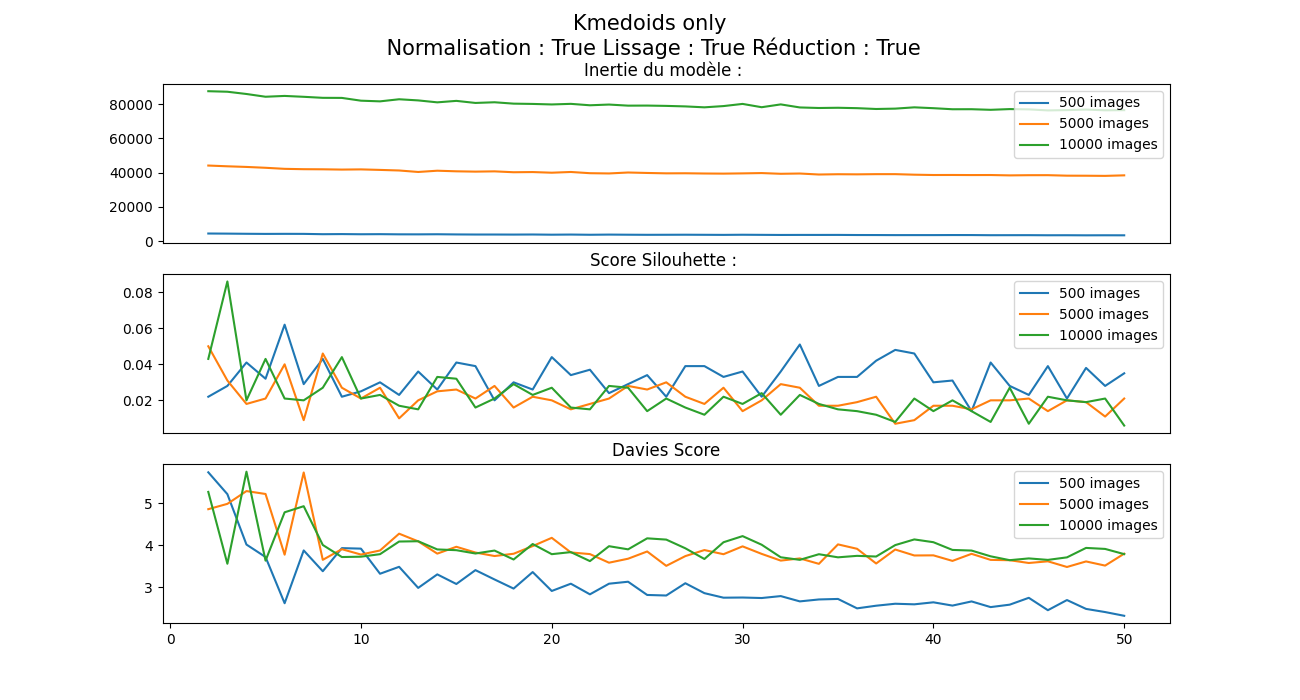
\includegraphics[width=\textwidth]{"./Images/Kmedoids_no_prepo.png"}
    \caption{Évolution des métriques de Kmedoids en fonction du nombre de clusters et de la taille du dataset}
    \label{fig:my_label}
\end{figure}

\begin{figure}[H]
    \centering
    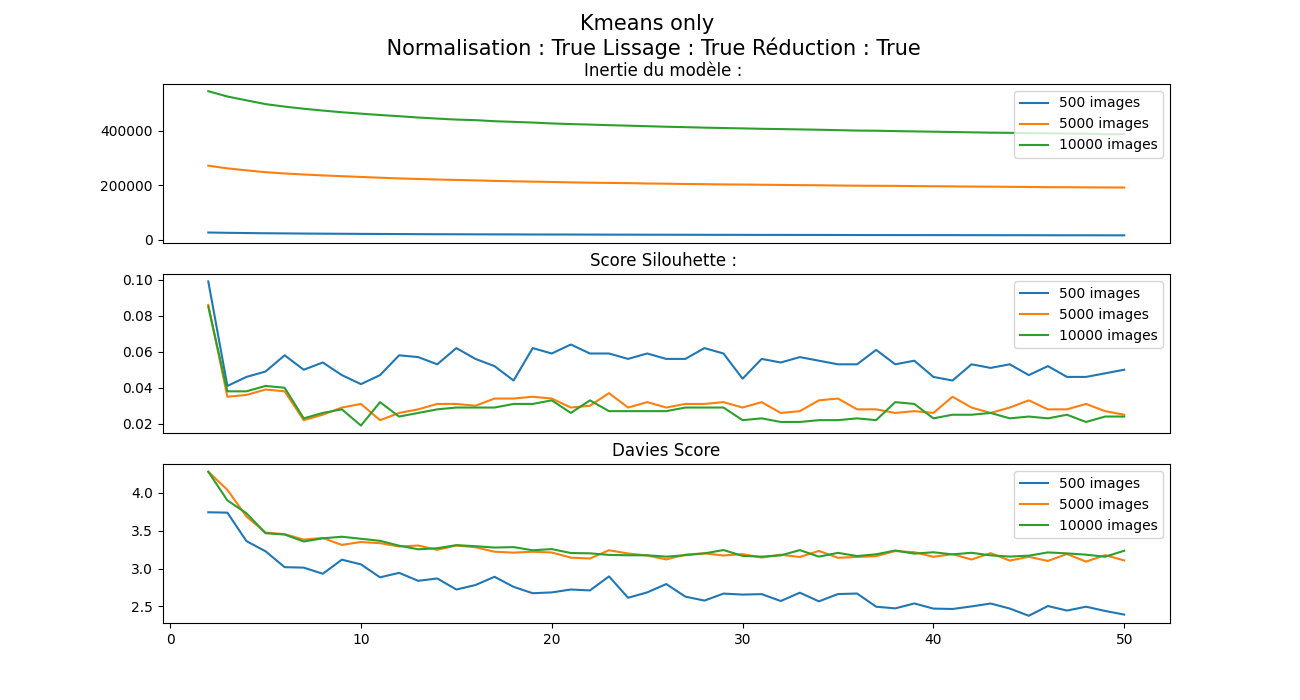
\includegraphics[width=\textwidth]{"./Images/Kmeans_no_prepro.png"}
    \caption{Évolution des métriques de Kmeans en fonction du nombre de clusters et de la taille du dataset}
    \label{fig:my_label}
\end{figure}


\textit{Au delà de 20000 images Kmedoids devenait beaucoup trop lent. Et augmenter encore le nombre d'images ne présente pas tant d'intérêt en terme de performances (du fait de la ressemblance des images, c'est pourquoi nous avons choisi ces tailles de base de données).}

\vspace{3mm}

Durant toutes ces itérations il a été notable que Kmeans est plus lent que Kmedoids, surtout sur de petites base de données. Leur temps de calcul respectif se rapprochent cependant avec l'augmentation du nombre de matrices considérées, et pour 10000 images Kmeans commence à passer devant Kmedoids. (Au delà Kmeans est d'ailleurs beaucoup plus rapide).

Ces courbes nous permettent de remarquer que l'inertie varie fortement selon le nombre d'images (ce qui est cohérent puisqu'elle repésente la distance intra cluster) et que les scores silouhette et Davies semblent regresser avec le nombre d'images. Cela tient probablement au fait que classifier un plus grand nombre de données avec un même nombre de clusters augmentent les chances de chevauchemen ou de mauvaise classifications.
\vspace{2mm}

\textit{Déterminer précisemment pourquoi s'avérerrait intéressant, mais la requête 'succint' concernant le rapport fait que nous avons choisi de ne pas nous y intéresser.}

\vspace{2mm}
Toute introduction étant, s'initier à la pratique du pré-traitement des bases de données est d'un grand intérêt. C'est pourquoi la partie suivante propose d'observer les conséquences de l'application de ce type d'algorithmes en amont des regroupements sur la qualité des clusterings de Kmeans et Kmedoids.


\section{Affiner avec du pré-traitement : des sommes}
\subsection{Principe}

Le principe est le suivant : pour chaque image nous sommons (après lissage et recadrage) la totalité des valeurs des pixels de chaque ligne et de chaque colonne.  Nous divisons ensuite par 22 le 2 vecteurs de taille 22 obtenus,  dont la valeurs de chaque coordonnées dépend du nombre de pixels blancs sur la ligne ou la colonne associée. Nous reconstruisons ensuite l'image à partir d'une somme terme à terme de ces deux vecteurs.

\begin{center}
    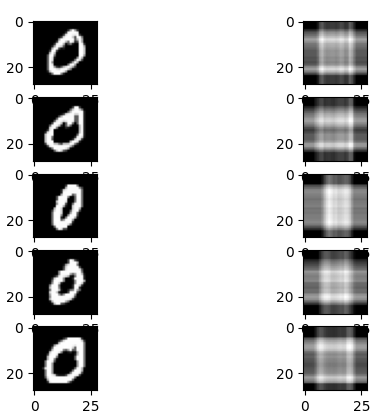
\includegraphics[width=0.6\textwidth]{./Images/spe_pre_pro_0.png}
    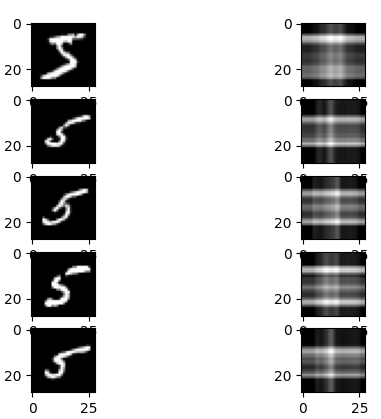
\includegraphics[width=0.6\textwidth]{./Images/spe_pre_pro_5.png}
\end{center}

\begin{center}
    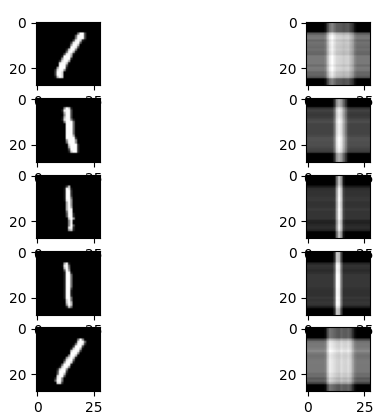
\includegraphics[width=0.6\textwidth]{./Images/spe_pre_pro_1.png}
    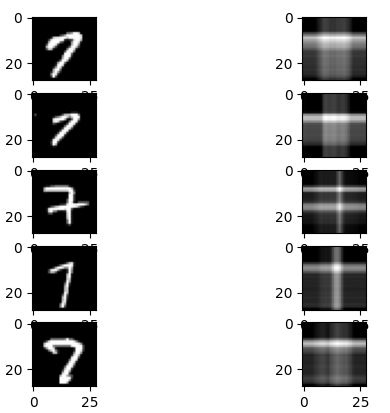
\includegraphics[width=0.6\textwidth]{./Images/spe_pre_pro_7.png}
\end{center}
Les chiffres restent 'humainement' reconnaissables et on remarque que les 7 et les 1 semblent plus facilement dissociables, ce qui est encourageant.

\subsection{Résultats}

Nous avons repris les mêmes configurations que celles de la partie précédente.
Les coubes obtenues pour Kmeans et Kmedoids sont les suivantes :

\begin{figure}[H]
    \centering
    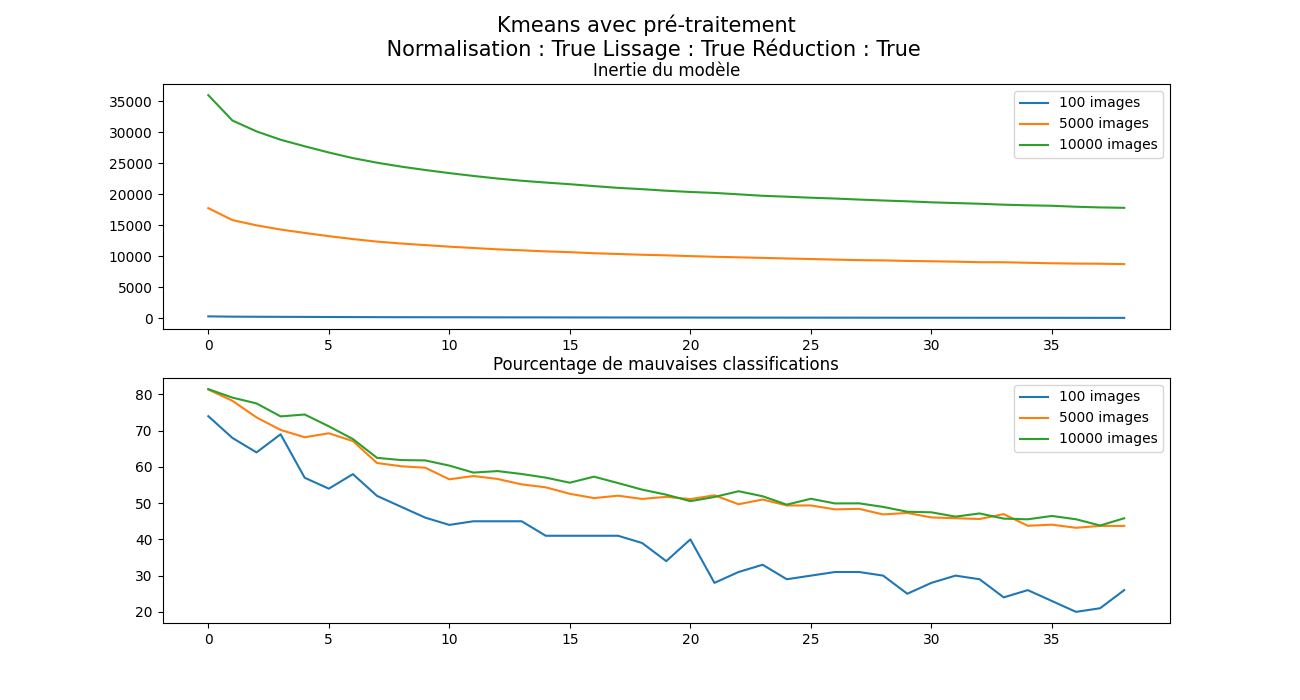
\includegraphics[width=\textwidth]{"./Images/Kmeans_prepro_err.png"}
    \caption{Inertie et erreur de classifications avec pré-traitement pour Kmeans}
\end{figure}

\begin{figure}[H]
    \centering
    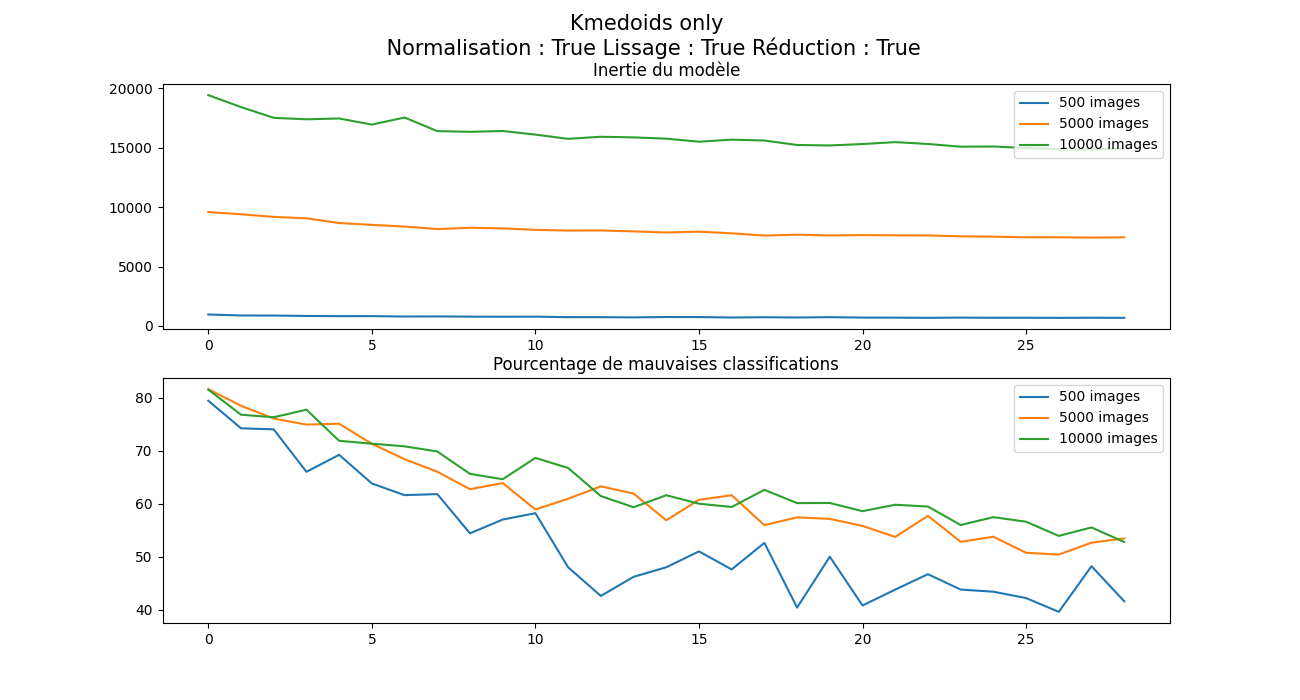
\includegraphics[width=\textwidth]{"./Images/Kmedoids_pre_pro_err.png"}
    \caption{Inertie et erreur de classifications avec pré-traitement pour Kmedoids}
    \label{fig:kmedoidspapapa}
\end{figure}
\vspace{2mm}

Nous remarquons que l'erreur de classification a diminuée dans  les deux cas (sachant que nous nous sommes arrêté à 30 clusters pour des raisons de temps de calcul) ! Ces résultat sont en accord avec les métriques de silouhette et de Davies qui présentaient également des chiffres plus favorables avec ce pré-traitement (nous avons choisi de ne pas afficher les courbes mais elles sont disponibles sur le github fourni en annexe).
Ces résultats encourageants tendent à envisager encore davantage d'algorithmes de discriminations des données (en re-lissant les images après traitement par exemple) pour observer si cette tendant continue de proposer de telles avancées ou ou non.

\subsection{Sur les limites}

Traiter les données en amont de la classification est cependant pas gratuit. Même si cela permet, lorsque bien pensé, d'améliorer les performances de la classification il faut cependant garder à l'esprit que le temps de calcul a parfois été augmenté d'un facteur non négligeable (pour Kmedoids il a été multiplié en moyenne par un facteur 4). Dans certain cas pratique cela peut se réveler problématique. 

Une autre bonne surprise est également à souligner : pour l'algorithme Kmeans nous avons obtenu que le temps moyen de détermination des barycentres a diminué de prêt d'un tiers avec du pré-traitement sur une base de données de 10 000 images, et qu'il est légèrement inférieur à celui sans pré-traitement pour une classification sur 1000 images. L'augmentation de la 'séparabilité' des données a permis d'accélérer la convergence de l'inertie et donc la temps passé à calculer les barycentres.

\section{Annexe}

\subsection{Codes}
L'ensemble des fonctions, modules et figures utilisés pour réaliser ou approfondir ce TP sont disponibles à l'adresse suivante : \href{https://github.com/Erwanlbv/P4_KM_MNIST.git}{\underline{\textit{https://github.com/Erwanlbv/P4\_KM\_MNIST.git}}}

\subsection{Références}

[1] : \url{http://www.xavierdupre.fr/app/mlstatpy/helpsphinx//c_clus/kmeans.html#id31}

[2] : \url{https://scikit-learn.org/stable/modules/generated/sklearn.metrics.silhouette_score.html}

\end{document}